%----------------------------------------------------------------------------------------
%	SLIDE 4.
%----------------------------------------------------------------------------------------
\begin{frame}
\frametitle{Implementation in Geant4 - Neutron beam}

\begin{exampleblock}{}
	\begin{itemize}
		\item Neutrons spawns behind the \texttt{NEBULA wall} block and fly towards it with a random position and inclination
		\item All neutrons are set to have $100$ MeV energy at the start
		\item A block called \texttt{Neutron E. Counter} counts neutrons passing through that volume and it's only there for debugging purposes
	\end{itemize}
\end{exampleblock}

\begin{figure}
	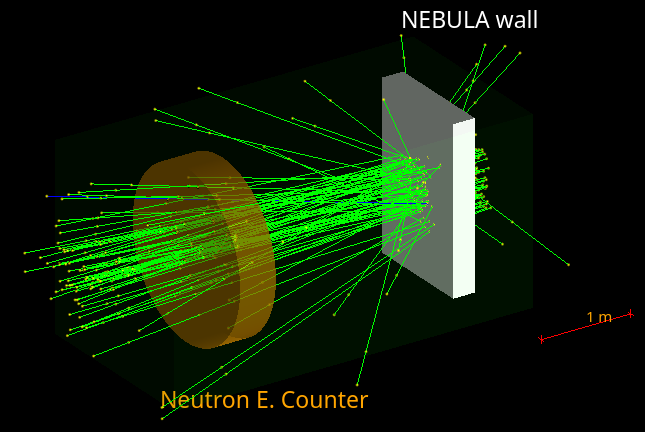
\includegraphics[width=0.5\textwidth]{images/nebula_3d.png}
\end{figure}

\end{frame}